\chapter{Least-squares Extrapolation} \label{ch:leastsquares}

Sometimes we don't want to fit data with a curve that is forced to pass through every point. We might instead assume there is a simple relation underneath the data and \textit{noise} scatters the data around this relation. For example, see figure~\ref{fig:ch4_purpose}.

\begin{figure}[H]
	\begin{center}
	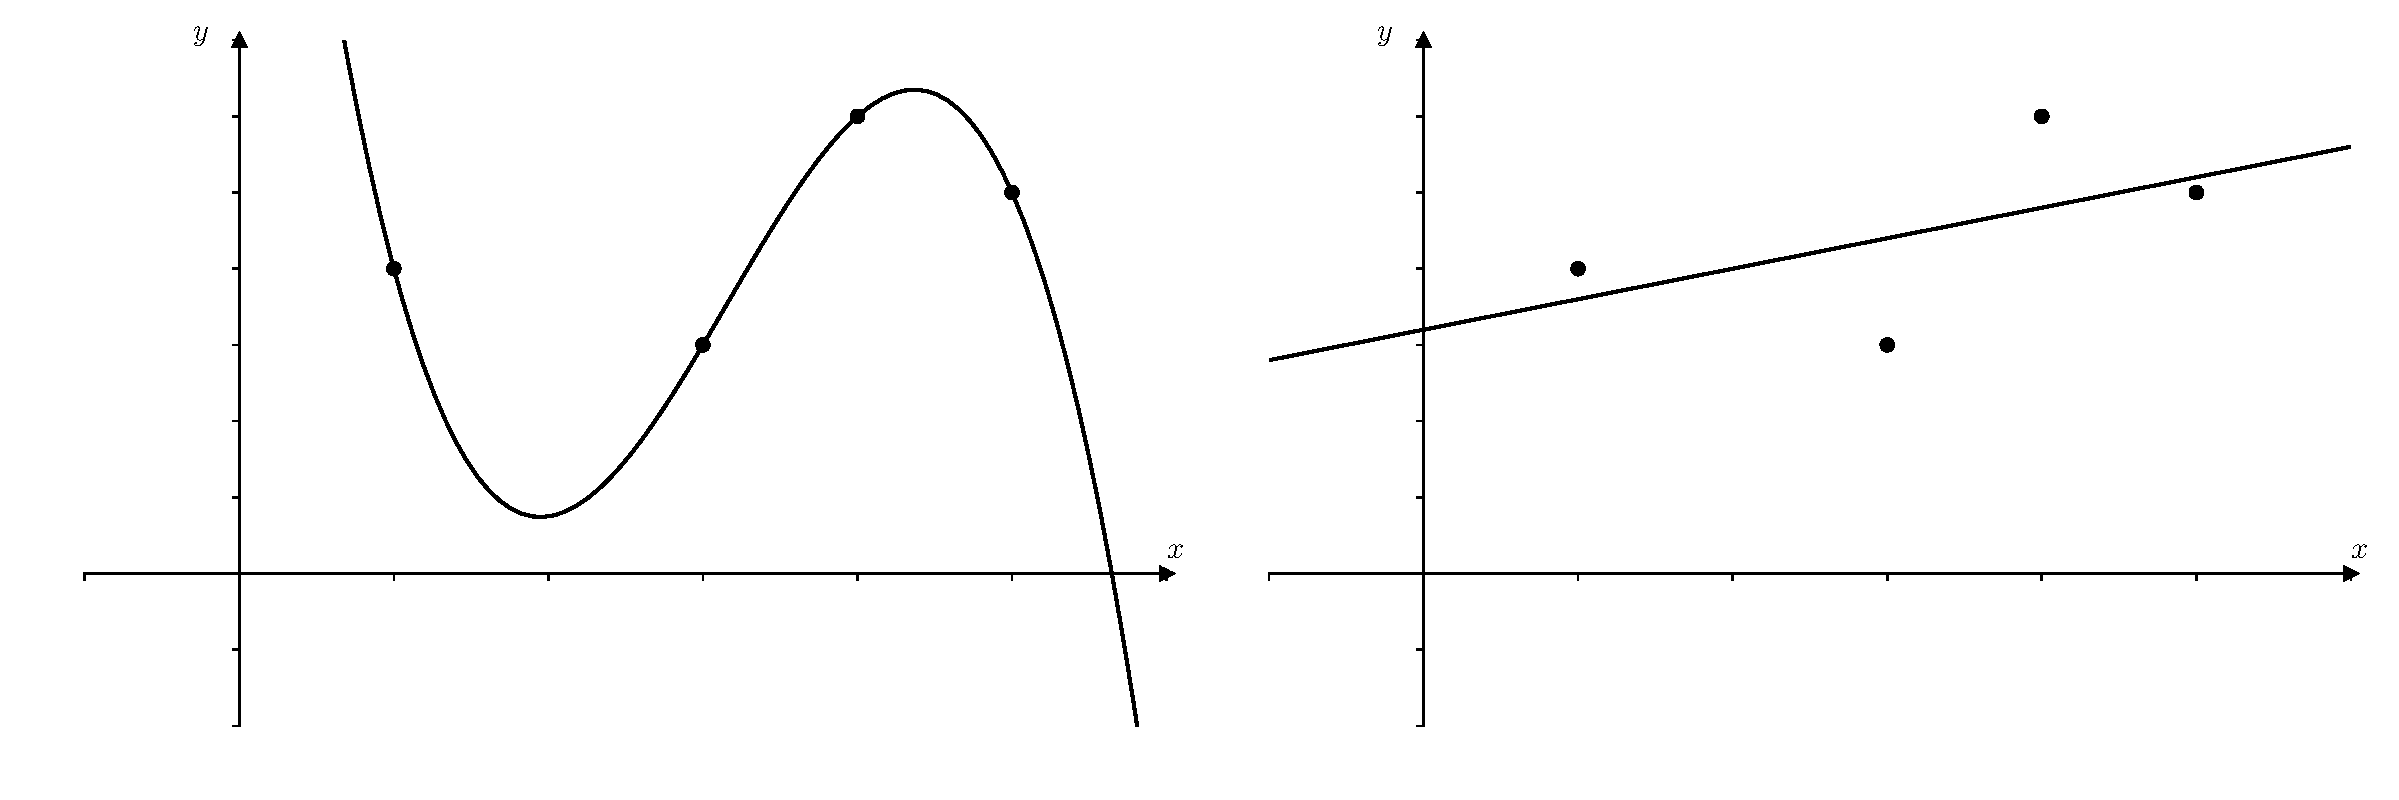
\includegraphics[width=\textwidth]{figures/ch4_least_squares_purpose.pdf} 
	  \caption{(Left) Lagrange polynomial passing through each point (right) simple line that roughly captures the trend of the data.} \label{fig:ch4_purpose}
	\end{center}
\end{figure}

If we see a rough trend in the data, we may want to predict what will happen outside of the data range. The Lagrange polynomial is bad at this, giving massive errors outside of the range of the given data. So, Lagrange is good for \textit{interpolation}, and in this chapter we will look at the method of least squares which is good for \textit{extrapolation}.

\section{Least-squares linear fitting}
Say you have $n+1$ data points $(x_k,y_k)$ for $k=0,1,2,\dots,n$. Imagine we want to \textit{fit} this data with a straight line. We want to find the best line $y=mx + b$, where best means to minimise the square of the \textit{residuals}:
\begin{align*}
r_k = y_k - y(x_k).
\end{align*}
Looking at figure~\ref{fig:ch4_defintion} you can see that the residual is the vertical distance between a data point and a straight line. So minimising the residuals is a way to choose a line that is closest to all the data points in some way. We minimise the square so that it doesn't matter whether the residual is positive or negative.

\begin{figure}[H]
	\begin{center}
	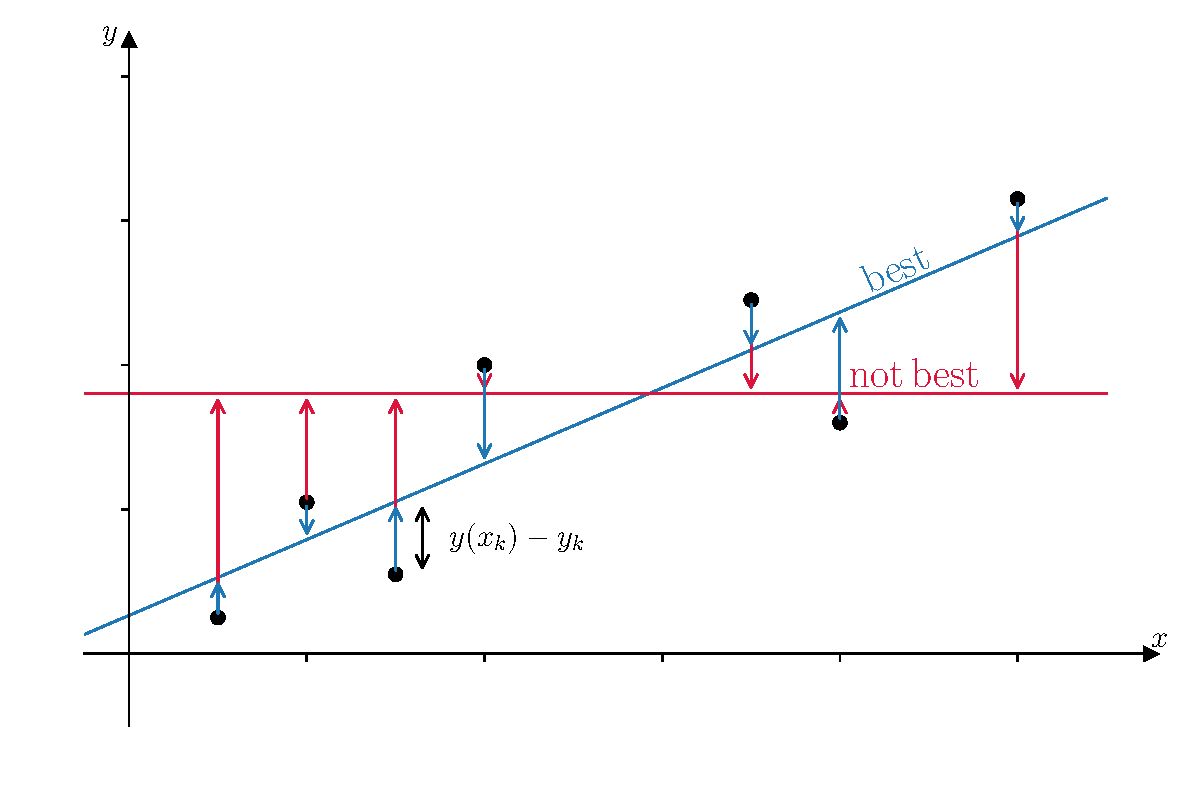
\includegraphics[width=0.7\textwidth]{figures/ch4_least_squares_defn.pdf} 
	  \caption{Two linear fits to the data points. The blue straight line minimises the collection of distances, $y(x_k)-y_k$, of each data point from the line. The red line is obviously worse.} \label{fig:ch4_defintion}
	\end{center}
\end{figure}

What are we changing when we say we are minimising the (square of the) residuals? We are adjusting a straight line, which means we are changing the slope ,$m$, and the vertical offset, $b$. So. let's define the sum of the square of the residuals as a two variable function in the variables $m$ and $b$
\begin{align*}
S(m,b) = \sum_{k=0}^n r_k^2 = \sum_{k=0}^n \left(y_k - y(x_k)\right)^2.
\end{align*}
This function is general for any fitting curve $y(x)$, but in this chapter we only use linear fits, so we can define the function $S$ as
\begin{align*}
S(m,b) = \sum_{k=0}^n \left(y_k - mx_k - b\right)^2.
\end{align*}

Recall that to find where a single-variable function, $f(x)$, is minimum (or maximum) you must find where its derivative is equal to zero. For multi-variate functions, we must find where its partial derivatives are zero. So we impose
\begin{align*}
\frac{\partial S}{\partial m} = 0 \\
\frac{\partial S}{\partial b} = 0.
\end{align*}
These partial derivatives are
\begin{align*}
\frac{\partial S}{\partial m} = \sum_{k=0}^n 2 r_k x_k = \sum_{k=0}^n 2 \left(y_k - mx_k - b\right) x_k\\
\frac{\partial S}{\partial b} = \sum_{k=0}^n 2 r_k = \sum_{k=0}^n 2 \left(y_k - mx_k - b\right)
\end{align*}
and so setting these to be zero, we must simultaneously solve
\begin{align}
\sum_{k=0}^n \left(y_k - mx_k - b\right) x_k = 0  \label{eq:dsdm}\\
\sum_{k=0}^n \left(y_k - mx_k - b\right) = 0 \label{eq:dsdb}
\end{align}


\exemple{\upline}
{
	Make a least-squares linear fit to the data: $\{ (1,1)$, $(2,3)$, $(3,2)$, $(5,3) \}$.
	
	\noindent We want $m$ and $b$ for $y(x) = mx + b$. The residuals are
	\begin{align*}
	r_0 &= 1 - m - b \\
	r_1 &= 3 - 2m - b \\
	r_2 &= 2 - 3m - b \\
	r_3 &= 3 - 5m - b
	\end{align*}
	
	The function to minimise is
	\begin{align*}
	S(m,b) &= r_0^2 + r_1^2 + r_2^2 + r_3^2\\
	&= 1 -   m -  b -   m +   m^2 +  mb -  b +  mb + b^2 + \\
	&  9 -  6m - 3b -  6m +  4m^2 + 2mb - 3b + 2mb + b^2 + \\
	&  4 -  6m - 2b -  6m +  9m^2 + 3mb - 2b + 3mb + b^2 + \\
	&  9 - 15m - 3b - 15m + 25m^2 + 5mb - 3b + 5mb + b^2.
	\end{align*}
	Finally, collecting all the terms we have
	\begin{align*}
	\boxed{S(m,b) = 23 - 56m -18b + 22mb + 39m^2 + 4b^2}
	\end{align*}
	The partial derivatives give
	\begin{align*}
	\frac{\partial S}{\partial m} &= -56 +22b + 78m = 0 \implies b=\frac{56-78m}{22} \\
	\frac{\partial S}{\partial b} &= -18 +22m + 8b = 0  \implies b=\frac{18-22m}{8}
	\end{align*}
	This eliminates $b$, allowing us to determine $m$
	\begin{align*}
	& \frac{56-78m}{22} = \frac{18-22m}{8} \\
	& 8(56 - 78m) = 22(18-22m)\\
	& 484m - 624m = 396 - 448 \\
	& m = \frac{52}{140} \sim 0.37
	\end{align*}
	and now plug this into either of the 2 equations for $b$
	\begin{align*}
	b \sim \frac{56-78\times 0.37}{22} \sim 1.23.
	\end{align*}
	So we have the least squares linear fit to the data
	\begin{align*}
	y = 0.37 x + 1.23.
	\end{align*}
}{\downline}

In this previous example we expanded the squares of residuals \textit{then} differentianted. It turns out to be easier to differentiate \textit{then} expand. Recall the partial derivative of $S$ with respect to $b$ gave us the condition
\begin{align*}
\sum_{k=0}^n \left(y_k - mx_k - b\right) = 0.
\end{align*}
This can be rearranged to
\begin{align*}
&\sum_{k=0}^n \left(y_k - mx_k\right) -  \sum_{k=0}^n b = 0 \\
&\sum_{k=0}^n \left(y_k - mx_k\right) -  (n+1) b = 0
\end{align*}
so that we have an expression for $b$
\begin{align*}
\boxed{b = \frac{1}{n+1}\sum_{k=0}^n \left(y_k - mx_k\right)}
\end{align*}

For the previous example with data $\{ (1,1)$, $(2,3)$, $(3,2)$, $(5,3) \}$, we have $n=3$, and this gives
\begin{align*}
b &= \frac{1}{4}\left( (1 - m) + (3-2m) + (2-3m) + (3-5m) \right) \\
&= \frac{9 - 11m}{4} = \frac{18 - 22m}{8}
\end{align*}
which is the same equation we had, but now we reached it faster.

The partial derivative with respect to $m$ gave us the condition
\begin{align*}
\sum_{k=0}^n x_k\left(y_k - mx_k - b\right) = 0.
\end{align*}
For this previous example this gives
\begin{align*}
& 1(1 - m - b) + 2(3-2m - b) + 3(2-3m - b) + 5(3-5m - b) = 0 \\
& 28 - 39m -11b = 0.
\end{align*}
This is the second equation that we got earlier, but now we reached it faster. Taking the derivatives before expanding is simpler because it removes the need to expand squared expressions.

But we can push this algebra further to create even simpler expressions for $b$ and $m$. So we start from the $b$ expression we just derived
\begin{align*}
b = \frac{1}{n+1}\sum_{k=0}^n y_k - m  \frac{1}{n+1}\sum_{k=0}^n x_k. 
\end{align*}
Now we note that the sum of a list of numbers, $x_k$, divided by how many numbers in that list is just the average value of the list, which we will denote $\bar{x}_k$. So we can write
\begin{align}
b = \bar{y}_k - m \bar{x}_k. \label{eq:offset1}
\end{align}
We insert this into equation~\ref{eq:dsdm} and clean things up
\begin{align*}
& \sum_{k=0}^n x_k\left(y_k - mx_k - b\right) = 0 \\
& \sum_{k=0}^n x_k\left(y_k - mx_k - \bar{y}_k + m \bar{x}_k\right) = 0 \\
& \sum_{k=0}^n \left( x_k \left(y_k - \bar{y}_k\right)   + m x_k\left(\bar{x}_k  - x_k\right) \right) = 0 \\
& \sum_{k=0}^n  x_k \left(y_k - \bar{y}_k\right)   + m \sum_{k=0}^n  x_k\left(\bar{x}_k  - x_k\right)  = 0.
\end{align*}
And this gives us an expression for $m$ that is independent of $b$
\begin{align*}
\boxed{  m   = \frac{\sum_{k=0}^n  x_k\left(\bar{y}_k - y_k\right)}{\sum_{k=0}^n  x_k \left(\bar{x}_k  - x_k \right) } }
\end{align*}
which can be plugged into equation~\ref{eq:offset1} to give an expression for $b$ that is independent of $m$
\begin{align*}
\boxed{b = \bar{y}_k - \bar{x}_k \frac{\sum_{k=0}^n  x_k\left(\bar{y}_k - y_k\right)}{\sum_{k=0}^n  x_k \left(\bar{x}_k  - x_k \right) } }
\end{align*}

These last two expressions are not necessarily easier to use in hand calculations, but they are very easy to code. A computer can take averages very easily, and so those two expressions might be more useful for creating a least-squares computer program.

\exemple{\upline}
{
	Make a least-squares linear fit to the data: $\{ (1,1)$, $(2,3)$, $(3,2)$, $(5,3) \}$. Same as the previous example, but with the new method.
	
	\noindent We need the averages of the $x_k$ and $y_k$:
	\begin{align*}
	\bar{x}_k &= \frac{1+2+3+5}{4} = \frac{11}{4} \\
	\bar{y}_k &= \frac{1+3+2+3}{4} = \frac{9}{4} 
	\end{align*}
	So we use the formula to calculate the slope
	\begin{align*}
	m   = \frac{1(\frac{9}{4}-1)+2(\frac{9}{4}-3)+3(\frac{9}{4}-2)+4(\frac{9}{4}-3)}{1(\frac{11}{4}-1)+2(\frac{11}{4}-2)+3(\frac{11}{4}-3)+5(\frac{11}{4}-5)} = \frac{-13/4}{-35/4} \sim 0.37
	\end{align*}
	Now we use this in the formula for the offset
	\begin{align*}
	b = \bar{y}_k - m \bar{x}_k \sim \frac{9}{4}  - 0.37 \times \frac{11}{4} \sim 1.23
	\end{align*}
	So we have the same least squares linear fit to the data
	\begin{align*}
	y = 0.37 x + 1.23.
	\end{align*}
	You decide whether this method is simpler or not.
}{\downline}


\section{Degree n polynomial least-squares}
We generalise the previous work by assuming a fitting polynomial of degree $p$:
\begin{align*}
y(x) = a_0 + a_1 x + a_2 x^2 + \dots + a_p x^p
\end{align*}
Then the sum of the square residuals function becomes a function of $p+1$ parameters
\begin{align*}
S(a_0, a_1, a_2, \dots, a_p) &= \sum_{k=0}^n \left( y(x_k) - y_k \right)^2 \\
&= \sum_{k=0}^n \left( a_0 + a_1 x_k + a_2 x_k^2 + \dots + a_p x_k^p - y_k \right)^2
\end{align*}
We now have $p+1$ partial derivatives to set to zero to find the minimised set of parameters:
\begin{align*}
\frac{\partial S}{\partial a_0} &= 2\sum_{k=0}^n \left( a_0 + a_1 x_k + a_2 x_k^2 + \dots + a_p x_k^p - y_k \right) \\
\frac{\partial S}{\partial a_1} &= 2\sum_{k=0}^n \left( a_0 + a_1 x_k + a_2 x_k^2 + \dots + a_p x_k^p - y_k \right) x_k \\
 & \,\vdots \\
\frac{\partial S}{\partial a_p} &= 2\sum_{k=0}^n \left( a_0 + a_1 x_k + a_2 x_k^2 + \dots + a_p x_k^p - y_k \right)  x_k^p
\end{align*}
Since all of these derivatives are set to zero, we can cancel the constant 2 in each equation, and we find a system of equations that is linear \textit{in the parameters}
\begin{align*}
 & \left(\sum_{k=0}^n 1\right) a_0 + \left(\sum_{k=0}^n x_k\right)a_1 +  \left(\sum_{k=0}^n  x_k^2\right)a_2 + \dots + \left(\sum_{k=0}^n  x_k^p \right)a_p  =  \sum_{k=0}^n y_k \\
 %
 & \left(\sum_{k=0}^n x_k\right) a_0 + \left(\sum_{k=0}^n x_k^2\right)a_1 +  \left(\sum_{k=0}^n  x_k^3\right)a_2 + \dots + \left(\sum_{k=0}^n  x_k^{p+1} \right)a_p  =  \sum_{k=0}^n y_k x_k \\
 %
 & \left(\sum_{k=0}^n x_k^2\right) a_0 + \left(\sum_{k=0}^n x_3\right)a_1 +  \left(\sum_{k=0}^n  x_k^2\right)a_4 + \dots + \left(\sum_{k=0}^n  x_k^{p+2} \right)a_p  =  \sum_{k=0}^n y_k x_k^2 \\
 %
 & \hspace{6cm} \vdots \\
 %
 & \left(\sum_{k=0}^n x_k^{p}\right) a_0 + \left(\sum_{k=0}^n x_k^{p+1}\right)a_1 +  \left(\sum_{k=0}^n  x_k^{p+2}\right)a_2 + \dots + \left(\sum_{k=0}^n  x_k^{2p} \right)a_p  =  \sum_{k=0}^n y_k  x_k^{p-1}
\end{align*}
This is better viewed as a matrix equation (and noting that $\dsum_{k=0}^n 1 = n+1$)
\begin{align*}
\begin{pmatrix}
n+1 & \dsum_{k=0}^n x_k & \dsum_{k=0}^n  x_k^2 & \cdots & \dsum_{k=0}^n  x_k^p   \\
%
\dsum_{k=0}^n x_k & \dsum_{k=0}^n x_k^2 & \dsum_{k=0}^n  x_k^3 & \cdots & \dsum_{k=0}^n  x_k^{p+1}   \\
%
\dsum_{k=0}^n x_k^2 & \dsum_{k=0}^n x_k^3 & \dsum_{k=0}^n  x_k^4 & \cdots & \dsum_{k=0}^n  x_k^{p+2}  \\
\vdots & \vdots & \vdots & \ddots & \vdots \\
%
\dsum_{k=0}^n x_k^p & \dsum_{k=0}^n x_k^{p+1} & \dsum_{k=0}^n  x_k^{p+2} & \cdots & \dsum_{k=0}^n  x_k^{2p}
\end{pmatrix}
%
\begin{pmatrix}
a_0 \\ a_1 \\ a_2 \\ \vdots \\ a_p
\end{pmatrix}
%
=
%
\begin{pmatrix}
\dsum_{k=0}^n y_k \\ \dsum_{k=0}^n y_k x_k \\ \dsum_{k=0}^n y_k x_k^2 \\ \vdots \\ \dsum_{k=0}^n y_k x_k^{p-1}
\end{pmatrix}
\end{align*}
Denoting this equation as $M \mathbf{a} = \mathbf{b}$, it can be shown (by a better mathematician) that $M$ is always an invertible matrix. So we can ``easily'' find the best-fit parameters with $\mathbf{a} = M^{-1} \mathbf{b}$.


\exemple{\upline}
{
	\noindent Make a 2nd degree polynomial least-squares fit to the data: $\{ (-1,2)$, $(2,-1)$, $(4,1)$, $(6,2) \}$. 
	
	\noindent In this problem $n=3$ ($n+1=4$ data points) and $p=2$ (degree 2 polynomial). We want a 2nd degree polynomial: $y(x) = a_0 + a_1 x + a_2 x^2$. The 2nd degree least-squares matrix equation, $M\mathbf{a} = \mathbf{b}$, is then
	\begin{align*}
	&
	\begin{pmatrix}
	4 & \dsum_{k=0}^3 x_k & \dsum_{k=0}^3  x_k^2 \\
	%
	\dsum_{k=0}^3 x_k & \dsum_{k=0}^3 x_k^2 & \dsum_{k=0}^3  x_k^3   \\
	%
	\dsum_{k=0}^3 x_k^2 & \dsum_{k=0}^3 x_k^3 & \dsum_{k=0}^3  x_k^4 
	\end{pmatrix}
	%
	\begin{pmatrix}
	a_0 \\ a_1 \\ a_2
	\end{pmatrix}
	%
	=
	%
	\begin{pmatrix}
	\dsum_{k=0}^n y_k \\ \dsum_{k=0}^n y_k x_k \\ \dsum_{k=0}^n y_k x_k^2 
	\end{pmatrix} \\
	%%
	%%
	%%
	\implies  M &=
	\begin{pmatrix}
	4 & -1+2+4+6 & 1+4+16+36 \\
	%
	-1+2+4+6 & 1+4+16+36 & -1+8+64+198   \\
	%
	1+4+16+36 & -1+8+64+198 & 1+16+256+1296
	\end{pmatrix} \\
	%
	&=
	\begin{pmatrix}
	4 & 11 & 57 \\
	%
	11 & 57 & 287   \\
	%
	57 & 287 & 1569
	\end{pmatrix} \\
	%%
	%%
	%%
	\text{and }  \mathbf{b} &=
	\begin{pmatrix}
	2-1+1+2 \\ 
	-2-2+4+12 \\ 
	2-4+16+72
	\end{pmatrix}
	%
	=
	\begin{pmatrix}
	4 \\ 
	12 \\ 
	86
	\end{pmatrix}
	\end{align*}
	The inverse of $M$ is
	\begin{align*}
	M^{-1} = \frac{1}{13112}\begin{pmatrix}
	7064 & -900 & 92 \\
	-900 & 3027 & -521 \\
	92 & -521 & 107
	\end{pmatrix}
	\end{align*}
	and therefore the polynomial coefficients (to 3 decimal places) are
	\begin{align*}
	\begin{pmatrix}
	a_0 \\ a_1 \\ a_2
	\end{pmatrix}
	%
	=
	%
	\frac{1}{13112}\begin{pmatrix}
	7064 & -900 &   92 \\
	-900 & 3027 & -521 \\
	  92 & -521 &  107
	\end{pmatrix}
	\begin{pmatrix}
	4 \\ 
	12 \\ 
	86
	\end{pmatrix}
	%%
	%%
	\sim
	\begin{pmatrix}
	 0.729 \\
	-0.921 \\
	 0.197
	\end{pmatrix}
	\end{align*}
	That is, the polynomial of degree 2 that minimizes the square of the residuals is
	\begin{align*}
	y(x) \sim 0.729 - 0.921 x + 0.197 x^2 
	\end{align*}
	This polynomial and the data plots are sketched below
	\begin{figure}[H]
	\centering
	\begin{tikzpicture}[
arr/.style = {very thick, draw=gray, -{Straight Barb[length=1mm]}},
domain=-2:7, samples=70
                        ]
	%\draw[very thin, color=green, step=0.2cm](-2,-3) grid (7,11);
	%\draw[color=cyan](-3,-3) grid (8,4);
	\filldraw[color=airforceblue] (-1,2) circle (3pt);
	\filldraw[color=airforceblue] (2,-1) circle (3pt);
	\filldraw[color=airforceblue] (4,1) circle (3pt);
	\filldraw[color=airforceblue] (6,2) circle (3pt);
	
	\draw[arr] (-3,0) -- (8, 0) node[below]{$x$};
	\draw[arr] (0,-3) -- (0,4) node[left]{$y$};
	% tick labels
	\foreach \x in {-2,-1,...,7}
	\draw (\x, 1pt) -- ++ (0,-1pt) node[below left] {$\x$};
	\foreach \y in {-2,-1,...,3}
	\draw (1pt, \y) -- ++ (-1pt, 0) node[below right] {$\y$};
	% function
	\draw[color=black, thick] plot (\x,{0.197*(\x)^2 - 0.921*\x + 0.729});
	\end{tikzpicture}
	\end{figure}
	Not so bad.
}{\downline}



\section{Non-polynomial least-squares}
We finish this chapter by showing that the linear fitting is more useful than you may realise. It can also be used to make non-linear fits (for example quadratic or exponential) by cleverly scaling the data first. 






%%%%%%%%%%%%%%%%%%%%%%%%%%%%
%%%%%%%%%%%%%%%%%%%%%%%%%%%%
%%%%%%%%%%%%%%%%%%%%%%%%%%%%
%%%% Exercises %%%%
%%%%%%%%%%%%%%%%%%%%%%%%%%%%
%%%%%%%%%%%%%%%%%%%%%%%%%%%%
%%%%%%%%%%%%%%%%%%%%%%%%%%%%
\exercises{
\section{Exercises}

\exercice{Given data $\{ (1,5), (3,6), (5,8), (7,9) \}$}

Make a least-squares linear fit to the given data (generated by $y=0.7x + 4$). 


\exercice{Given data $\{ (1,7), (3,10), (4,12), (5,14),(7,18) \}$}

Make a least-squares linear fit to the given data (generated by $y=2.2x + 3$). 


\exercice{Given data $\{ (1,5), (2,11), (4,33), (5,59) \}$}

Make a least-squares exponential fit to the given data (generated by $y=3e^{0.6x}$). 

\exercice{Given data $\{ (1,1), (3,2), (5,5), (7,9), (8,12) \}$}

Make a least-squares exponential fit to the given data (generated by $y=e^{0.3x}$). 

\exercice{Given data $\{ (1,1), (3,3), (5,8), (7,15) \}$}

Make a least-squares quadratic fit to the given data (generated by $y=3x^2$). 

\exercice{Given data $\{ (1,10), (2,40), (3,89), (4,159), (6,359) \}$}

Make a least-squares quadratic fit to the given data (generated by y=$10x^2$). 
}